\documentclass[12pt]{mwart}

\usepackage{polski}
\usepackage[utf8]{inputenc}
\usepackage{mathtools,amsthm,amssymb,icomma,upgreek,xfrac,graphics,scrextend,float,tabularx,hyperref,multicol,array,caption}
\usepackage[table,xcdraw]{xcolor}

\mathtoolsset{mathic}
\raggedbottom
\graphicspath{ {./images/} }
\renewcommand{\refname}{Źródła}
\captionsetup{justification=raggedright,singlelinecheck=true}


\begin{document}
	
	\begin{center}
		{\Large\textbf{Statystyka stosowana}}
	\end{center}
	\begin{center}
		Raport 1
	\end{center}
	
	\noindent Temat: \ \textbf{Analiza wybranego zbioru danych}\\
	Imię i Nazwisko prowadzącego kurs: \ \textbf{Mgr Katarzyna Maraj-Zygmąt}	\newline\newline
	
	
	\noindent\begin{tabularx}{\textwidth}{|X |X|}
		\hline
		\begin{center}
			Imię i Nazwisko,\\ nr indeksu
		\end{center} &  \begin{center}
			Szymon Malec,\\ 262276
		\end{center}\\\hline
		Wydział & Wydział matematyki, W13 \\\hline
		Dzień i godzina zajęć: & Wtorek,\vphantom{ $11^{1^{5}}$} $7^{30}$\\\hline
		Kod grupy ćwiczeniowej & T00-64c \\\hline
		Data oddania raportu: & 10.05.2022 \\\hline
		\textbf{Ocena końcowa} &\\\hline
	\end{tabularx}\newline\newline
	
	\noindent\textbf{Adnotacje i uwagi:}
	
	\newpage
	
	
	\section{Wstęp}
	
	Celem raportu jest wykorzystanie dotychczas poznanych narzędzi statystycznych do zbadania wybranego zbioru danych. W dalszej części przeanalizuję pewną grupę danych w celu wyznaczenia ich podstawowych charakterystyk, znalezienia ich rozkładu oraz sprawdzenia czy dane w jakiś sposób ze sobą korelują.


	\section{Opis danych\textsuperscript{\cite{dane}}}
	
	Do opracowania wybrałem zbiór danych zawierający 6292 pomiary wzrostu i wagi 3333 zawodników startujących w mistrzostwach świata w hokeju na lodzie mężczyzn (IIHF World Championship) w latach 2001-2016. Ponieważ dane pochodzą z 16 turniejów, niektórzy zawodnicy, którzy startowali więcej niż jeden raz, powtarzają się. Nie pomijamy jednak tych powtórzeń, ponieważ mają one wpływ na całkowity rozkład wysokości i wagi osób startujących w zawodach.
	
	\begin{figure}[H]
		\centering
		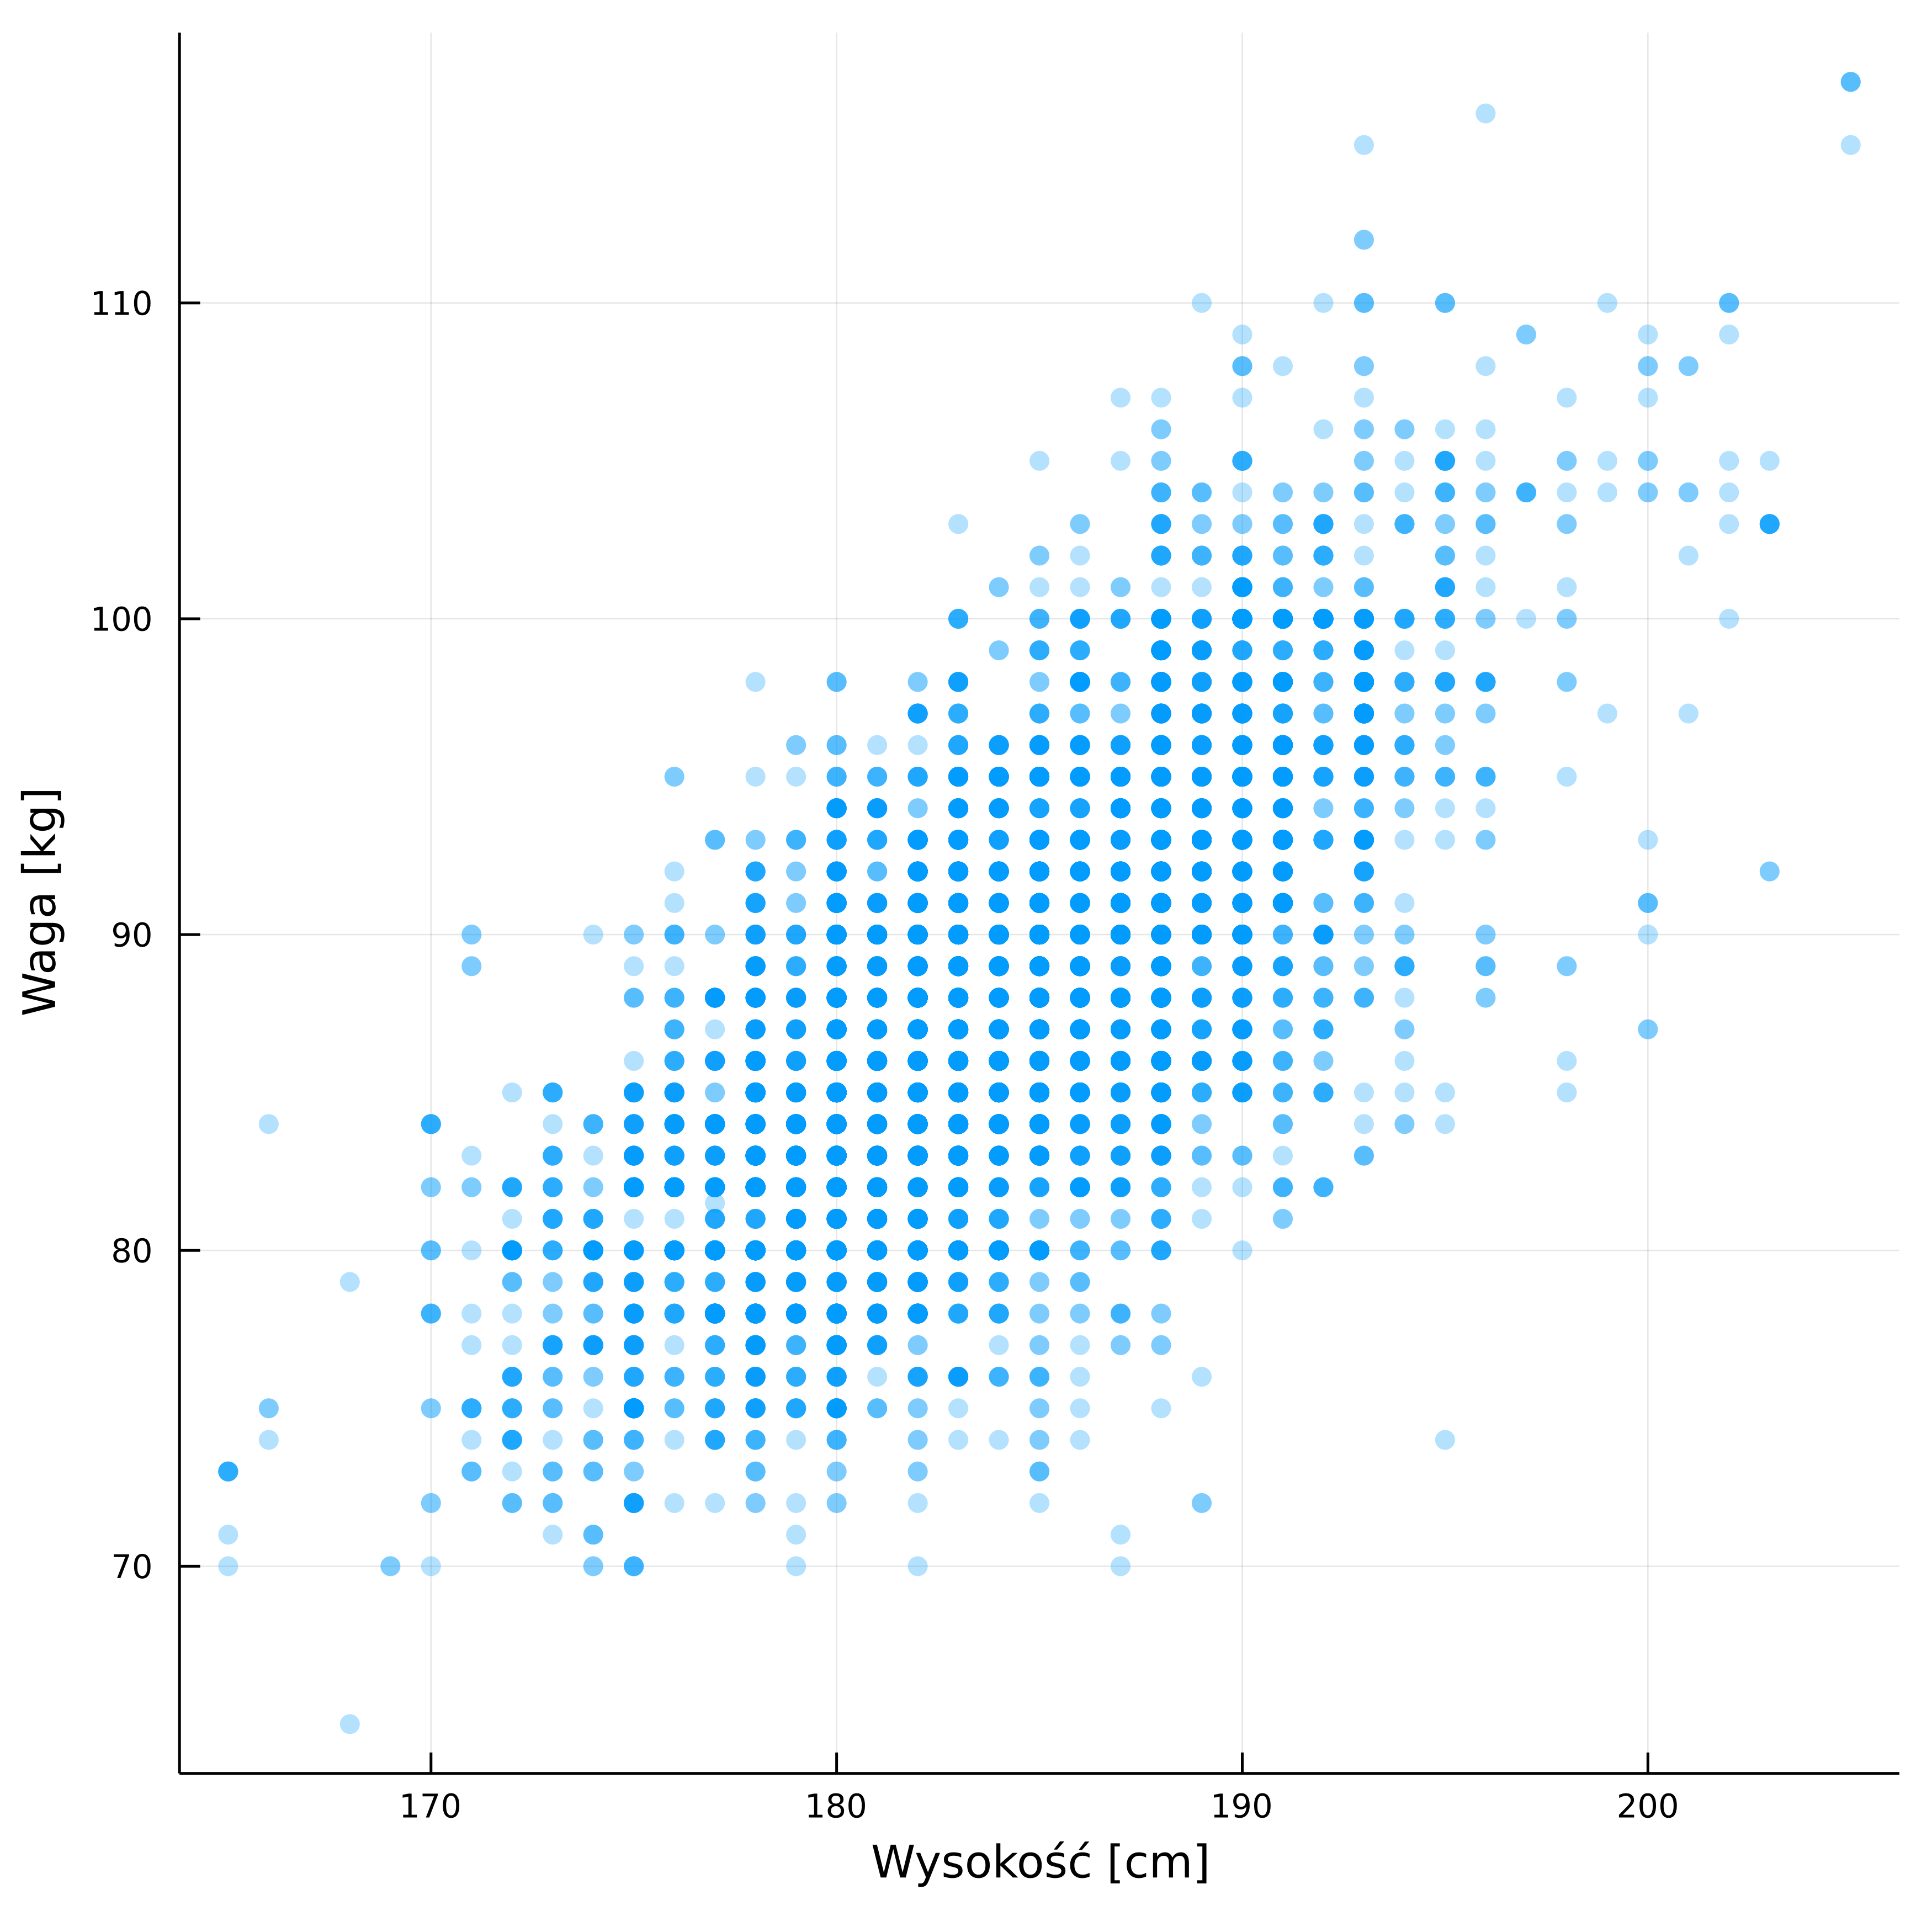
\includegraphics[scale=0.1]{images/scatter.png}
		\caption{Wykres punktowy wysokości od wagi zawodnika.}
	\end{figure}
	
	\newpage
	\begin{table}[H]
	\begin{multicols}{2}
		\begin{table}[H]
			\centering
			\begin{tabular}{|c|c|}
				\hline
				\textbf{Wysokość [cm]} & \textbf{Waga [kg]} \\ \hline
				185 & 84 \\ \hline
				188 & 86 \\ \hline
				182 & 95 \\ \hline
				178 & 85 \\ \hline
				175 & 88 \\ \hline
				193 & 93 \\ \hline
				176 & 84 \\ \hline
				183 & 91 \\ \hline
				180 & 85 \\ \hline
				178 & 86 \\ \hline
				187 & 93 \\ \hline
				185 & 80 \\ \hline
				198 & 95 \\ \hline
				175 & 77 \\ \hline
				178 & 75 \\ \hline
				181 & 85 \\ \hline
				194 & 95 \\ \hline
				186 & 87 \\ \hline
				184 & 86 \\ \hline
				178 & 92 \\ \hline
				175 & 90 \\ \hline
				187 & 86 \\ \hline
				180 & 75 \\ \hline
				188 & 84 \\ \hline
				182 & 88 \\ \hline
				182 & 88 \\ \hline
				175 & 88 \\ \hline
				188 & 90 \\ \hline
				190 & 96 \\ \hline
				181 & 86 \\ \hline
				196 & 98 \\ \hline
				190 & 100 \\ \hline
				185 & 95 \\ \hline
				186 & 88 \\ \hline
				180 & 76 \\ \hline
				176 & 72 \\ \hline
				183 & 82 \\ \hline
				173 & 85 \\ \hline
				185 & 87 \\ \hline
				182 & 84 \\ \hline
			\end{tabular}
		\end{table}
		\columnbreak
		\begin{table}[H]
			\centering
			\begin{tabular}{|c|c|}
				\hline
				\textbf{Wysokość [cm]} & \textbf{Waga [kg]} \\ \hline
				191 & 94 \\ \hline
				182 & 92 \\ \hline
				184 & 90 \\ \hline
				182 & 92 \\ \hline
				192 & 90 \\ \hline
				187 & 80 \\ \hline
				179 & 88 \\ \hline
				180 & 78 \\ \hline
				178 & 78 \\ \hline
				188 & 84 \\ \hline
				180 & 78 \\ \hline
				178 & 83 \\ \hline
				183 & 91 \\ \hline
				182 & 78 \\ \hline
				185 & 87 \\ \hline
				193 & 97 \\ \hline
				179 & 83 \\ \hline
				185 & 82 \\ \hline
				185 & 83 \\ \hline
				184 & 92 \\ \hline
				186 & 80 \\ \hline
				184 & 89 \\ \hline
				178 & 83 \\ \hline
				178 & 88 \\ \hline
				185 & 87 \\ \hline
				192 & 99 \\ \hline
				190 & 92 \\ \hline
				191 & 92 \\ \hline
				193 & 97 \\ \hline
				183 & 89 \\ \hline
				183 & 82 \\ \hline
				184 & 84 \\ \hline
				177 & 80 \\ \hline
				177 & 77 \\ \hline
				178 & 88 \\ \hline
				178 & 81 \\ \hline
				181 & 84 \\ \hline
				185 & 90 \\ \hline
				181 & 88 \\ \hline
				178 & 86 \\ \hline
			\end{tabular}
		\end{table}
	\end{multicols}
	\caption{Przykładowe dane.}
	\end{table}
	
	\begin{figure}[H]
		\centering
		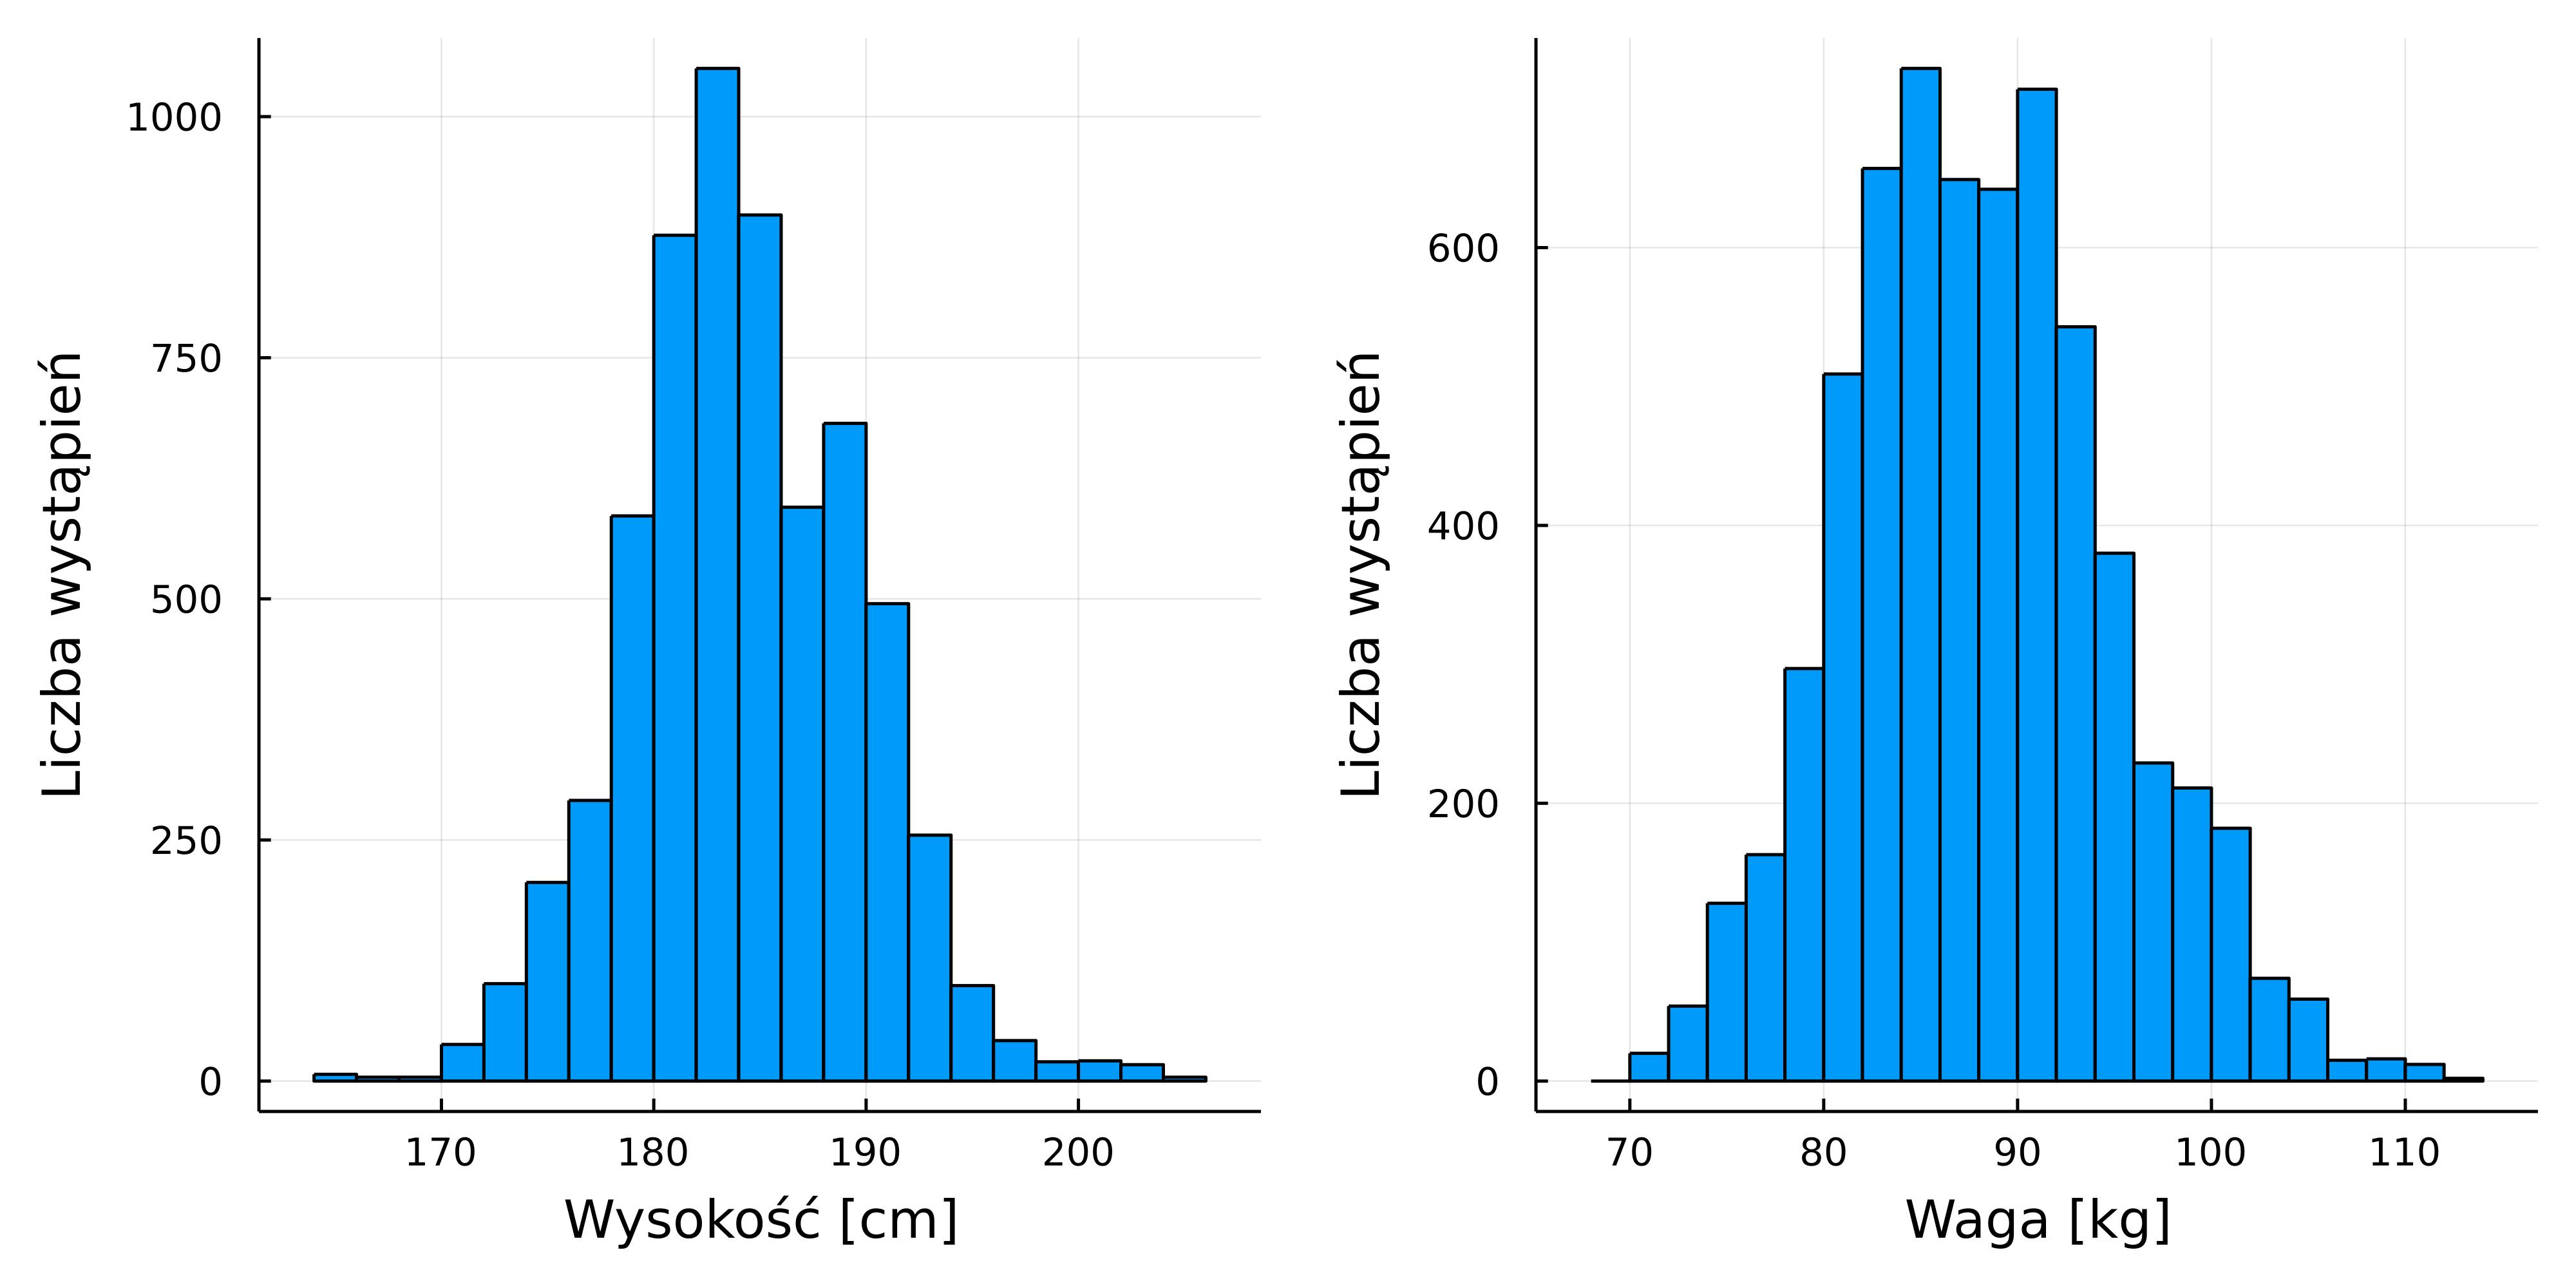
\includegraphics[scale=0.1]{images/histograms.png}
		\caption{Po lewej histogram z wysokości, po prawej z wag.}
	\end{figure}
	
	
	\section{Analiza rozkładów wysokości i wagi zawodników}
	
	Dane mają charakter dyskretny, co jest spowodowane dokładnością pomiarów wynoszącą 1cm w przypadku wysokości i 1kg w przypadku wagi. Rzeczywiste wartości mają jednak rozkład ciągły. Rozkład dyskretny, który otrzymamy z danych, będzie można traktować jako przybliżenie rzeczywistego rozkładu ciągłego.
	
	Niech $ x_1, x_2, \dots, x_n $ oznaczają dane posortowane rosnąco. Liczba danych wynosi $ n = 6292 $. Obliczamy podstawowe charakterystyki, w celu otrzymania więcej informacji o rozkładach.
	
	\begin{table}[H]
		\centering
		\begin{tabular}{| m{3.4cm} | c | m{2cm} | m{2cm} |}
			\hline & & & \\[-1em]
			\textbf{Charakterystyka} & \textbf{Wzór} & \textbf{Wartość dla \mbox{wysokości}} & \textbf{Wartość dla wagi}
			\\[-1em] & & & \\\hline & & & \\[-1em]
			Średnia \mbox{arytmetyczna} & $\bar{x}=\frac{1}{n}\sum\limits_{i=1}^{n}x_i$ & 183,8 & 87,6 
			\\[-1em] & & & \\\hline & & & \\[-1em]
			Wariancja & $S^2=\frac{1}{n-1}\sum\limits_{i=1}^{n}(x_i-\bar{x})^2$ & 29 & 48,5
			\\[-1em] & & & \\\hline & & & \\[-1em]
			Odchylenie \mbox{standardowe} & $S=\sqrt{S^2}$ & 5,4 & 7
			\\[-1em] & & & \\\hline & & & \\[-1em]
			Mediana & ------ & 183 & 87
			\\[-1em] & & & \\\hline & & & \\[-1em]
			Kwartyl $Q_1$ & ------ & 180 & 83
			\\[-1em] & & & \\\hline & & & \\[-1em]
			Kwartyl $Q_3$ & ------ & 188 & 92
			\\[-1em] & & & \\\hline & & & \\[-1em]
			Rozstęp & $R = x_n - x_1$ & 40 & 52
			\\[-1em] & & & \\\hline & & & \\[-1em]
			Rozstęp międzykwartylowy & $IQR = Q_3 - Q_1$ & 8 & 9
			\\[-1em] & & & \\\hline & & & \\[-1em]
			Współczynnik zmienności & $V=\frac{S}{\bar{x}}$ & 0,029 & 0,079
			\\[-1em] & & & \\\hline
		\end{tabular}
		\caption{Najważniejsze charakterystyki obliczone dla danych}
	\end{table}

	Na powyższej tabeli możemy zobaczyć, że w obu przypadkach średnia arytmetyczna jest zbliżona do mediany, co wskazuje, że rozkłady te są symetryczne. Widzimy także, że odchylenie standardowe dla wag jest trochę większe niż dla wysokości, zatem te pierwsze dane mają nieco większy rozrzut. Wskazuje na to także rozstęp międzykwartylowy. 
%	Wymienione obserwacje widoczne są również na wykresie pudełkowym, przy czym w przypadku wysokości widoczne jest
	
	\begin{figure}[H]
		\centering
		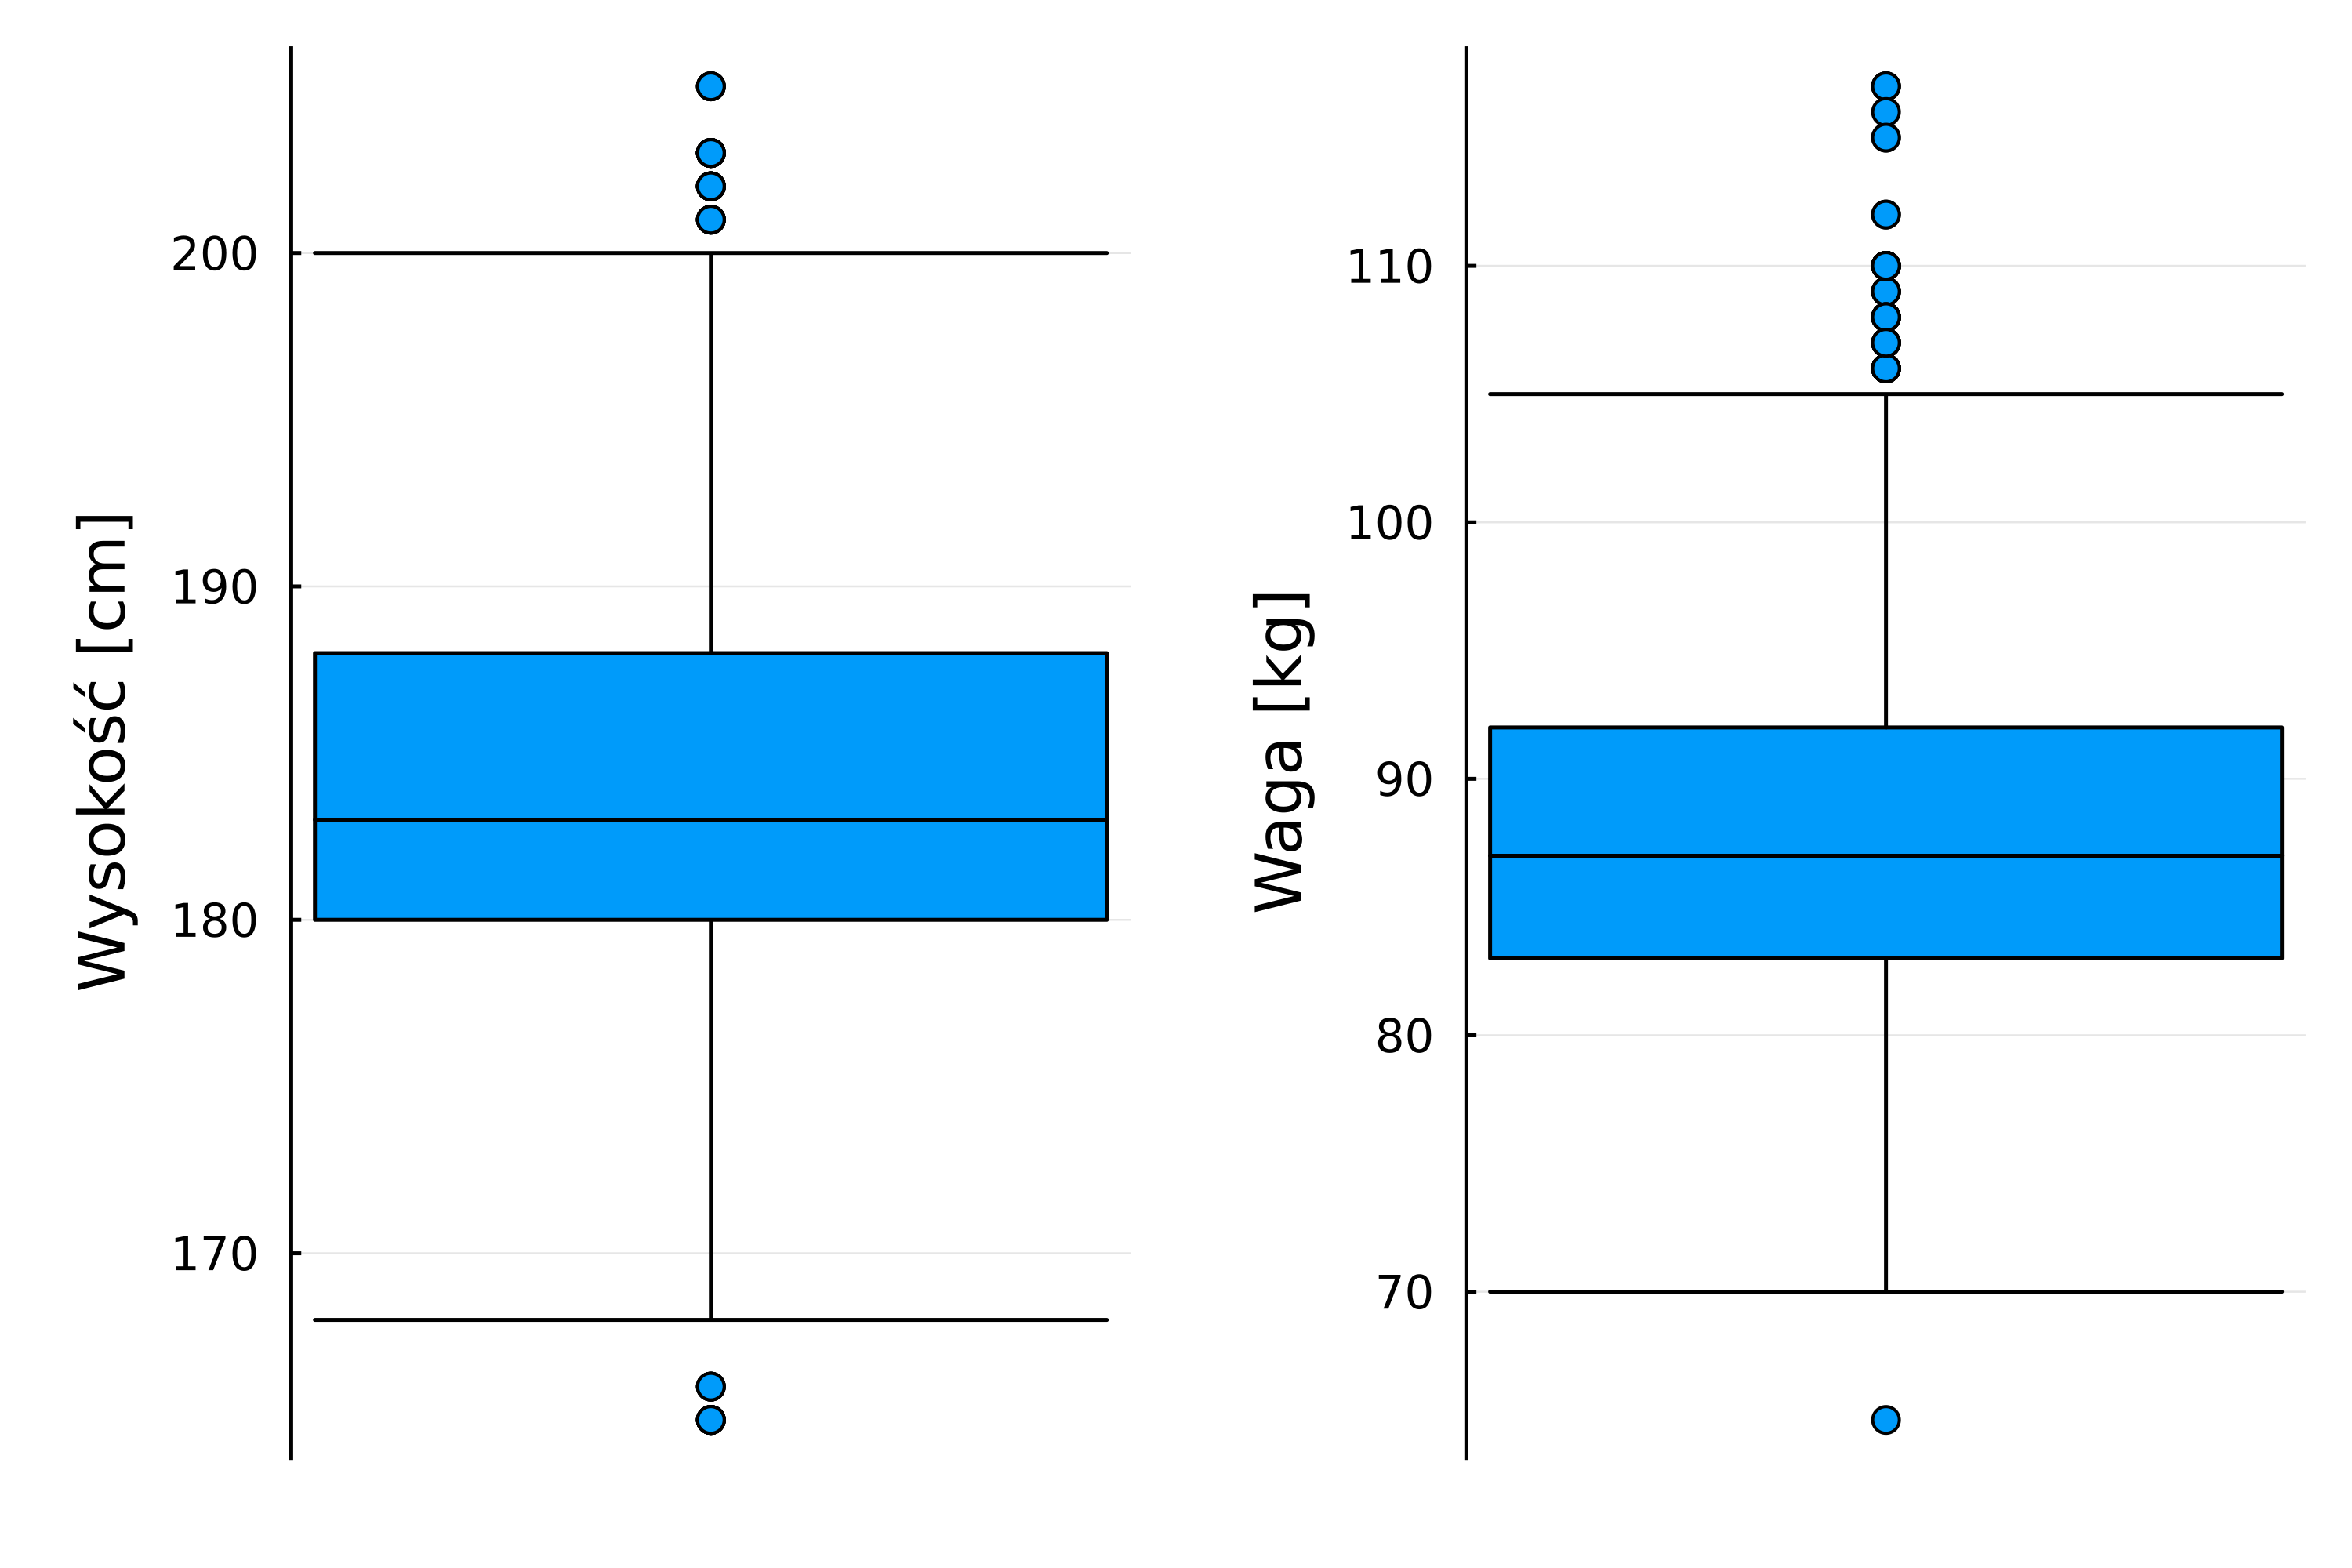
\includegraphics[scale=0.1]{images/boxplot.png}
		\caption{Wykresy pudełkowe dla badanych danych.}
	\end{figure}
	
	\newpage
	Korzystając z pakietu KernelDensity dostępnego w Julii możemy znaleźć gęstość empiryczną dla naszych danych, która będzie przybliżeniem gęstości rozkładu, z którego te dane pochodzą.
	
	\begin{figure}[H]
		\centering
		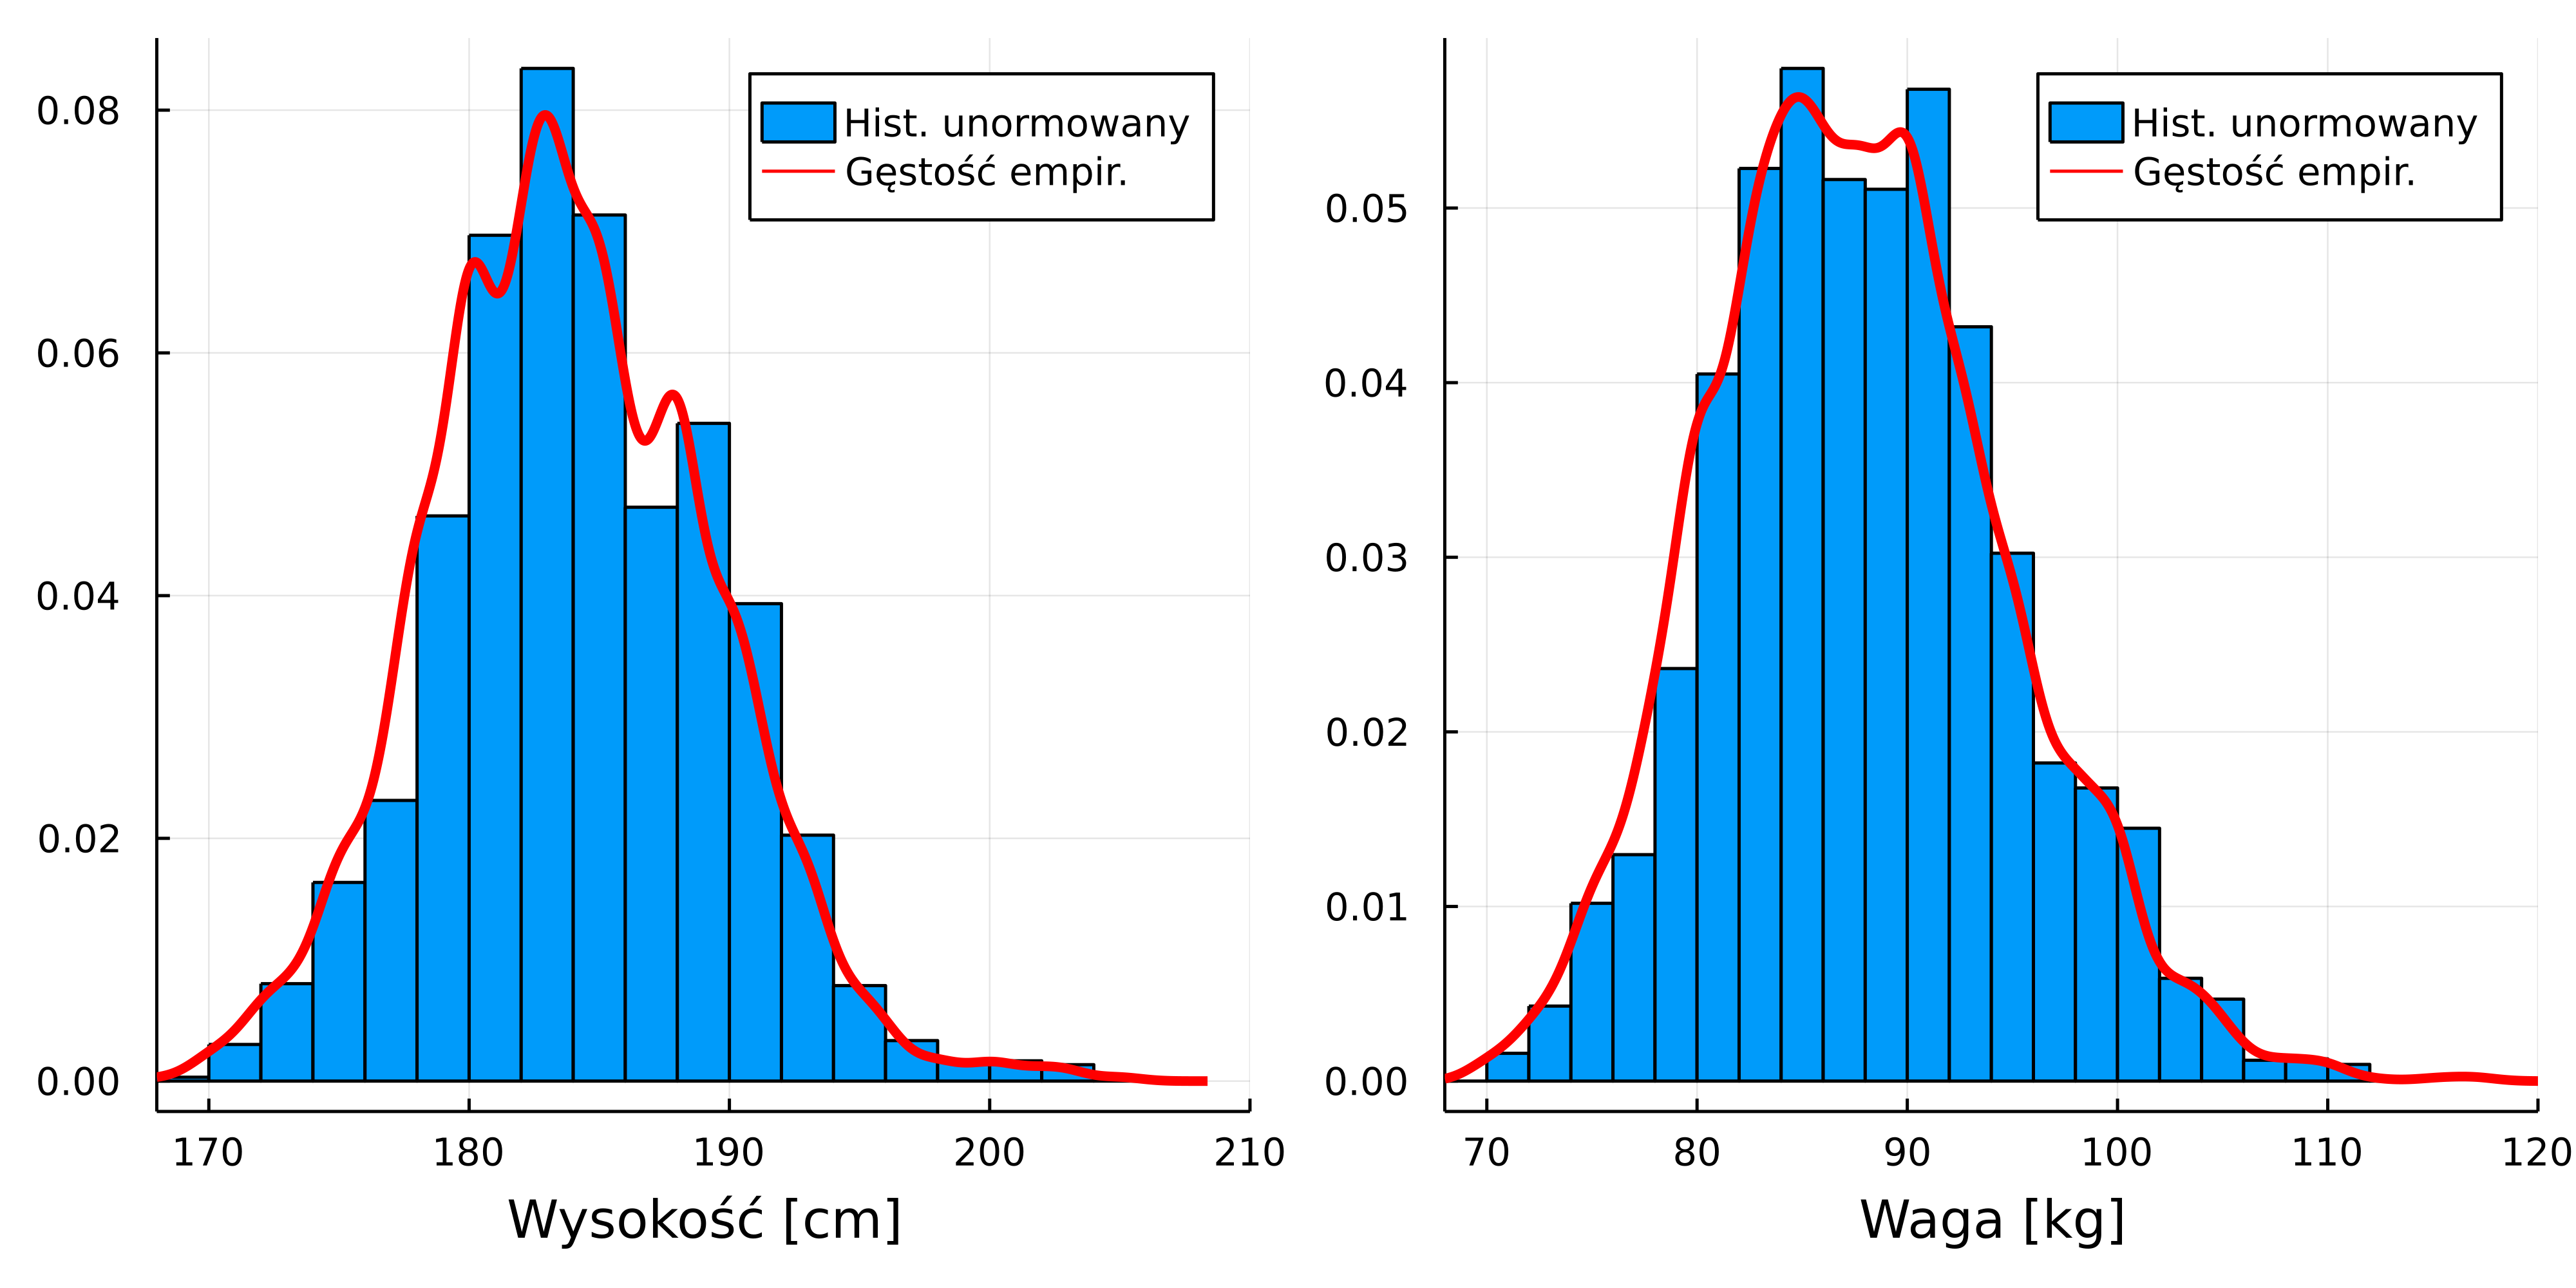
\includegraphics[scale=0.1]{images/density.png}
		\caption{Porównanie unormowanych histogramów i gęstości empirycznych, po lewej dla wysokości, po prawej dla wagi.}
	\end{figure}

	\noindent Jak możemy zobaczyć na powyższych wykresach, gęstości empiryczne pokrywają się z histogramami. Dodatkowo zauważamy, że w obu przypadkach krzywe gęstości przypominają krzywą Gaussa. Aby sprawdzić czy w rzeczywistości nasze dane pochodzą z rozkładu normalnego, porównamy wykresy gęstości empirycznych z wykresami gęstości teoretycznych rozkładu $\mathcal{N}(\mu, \sigma)$, gdzie pod $\mu$ podstawimy obliczone wcześniej średnie arytmetyczne, a pod $\sigma$ odchylenia standardowe.
	
	\begin{figure}[H]
		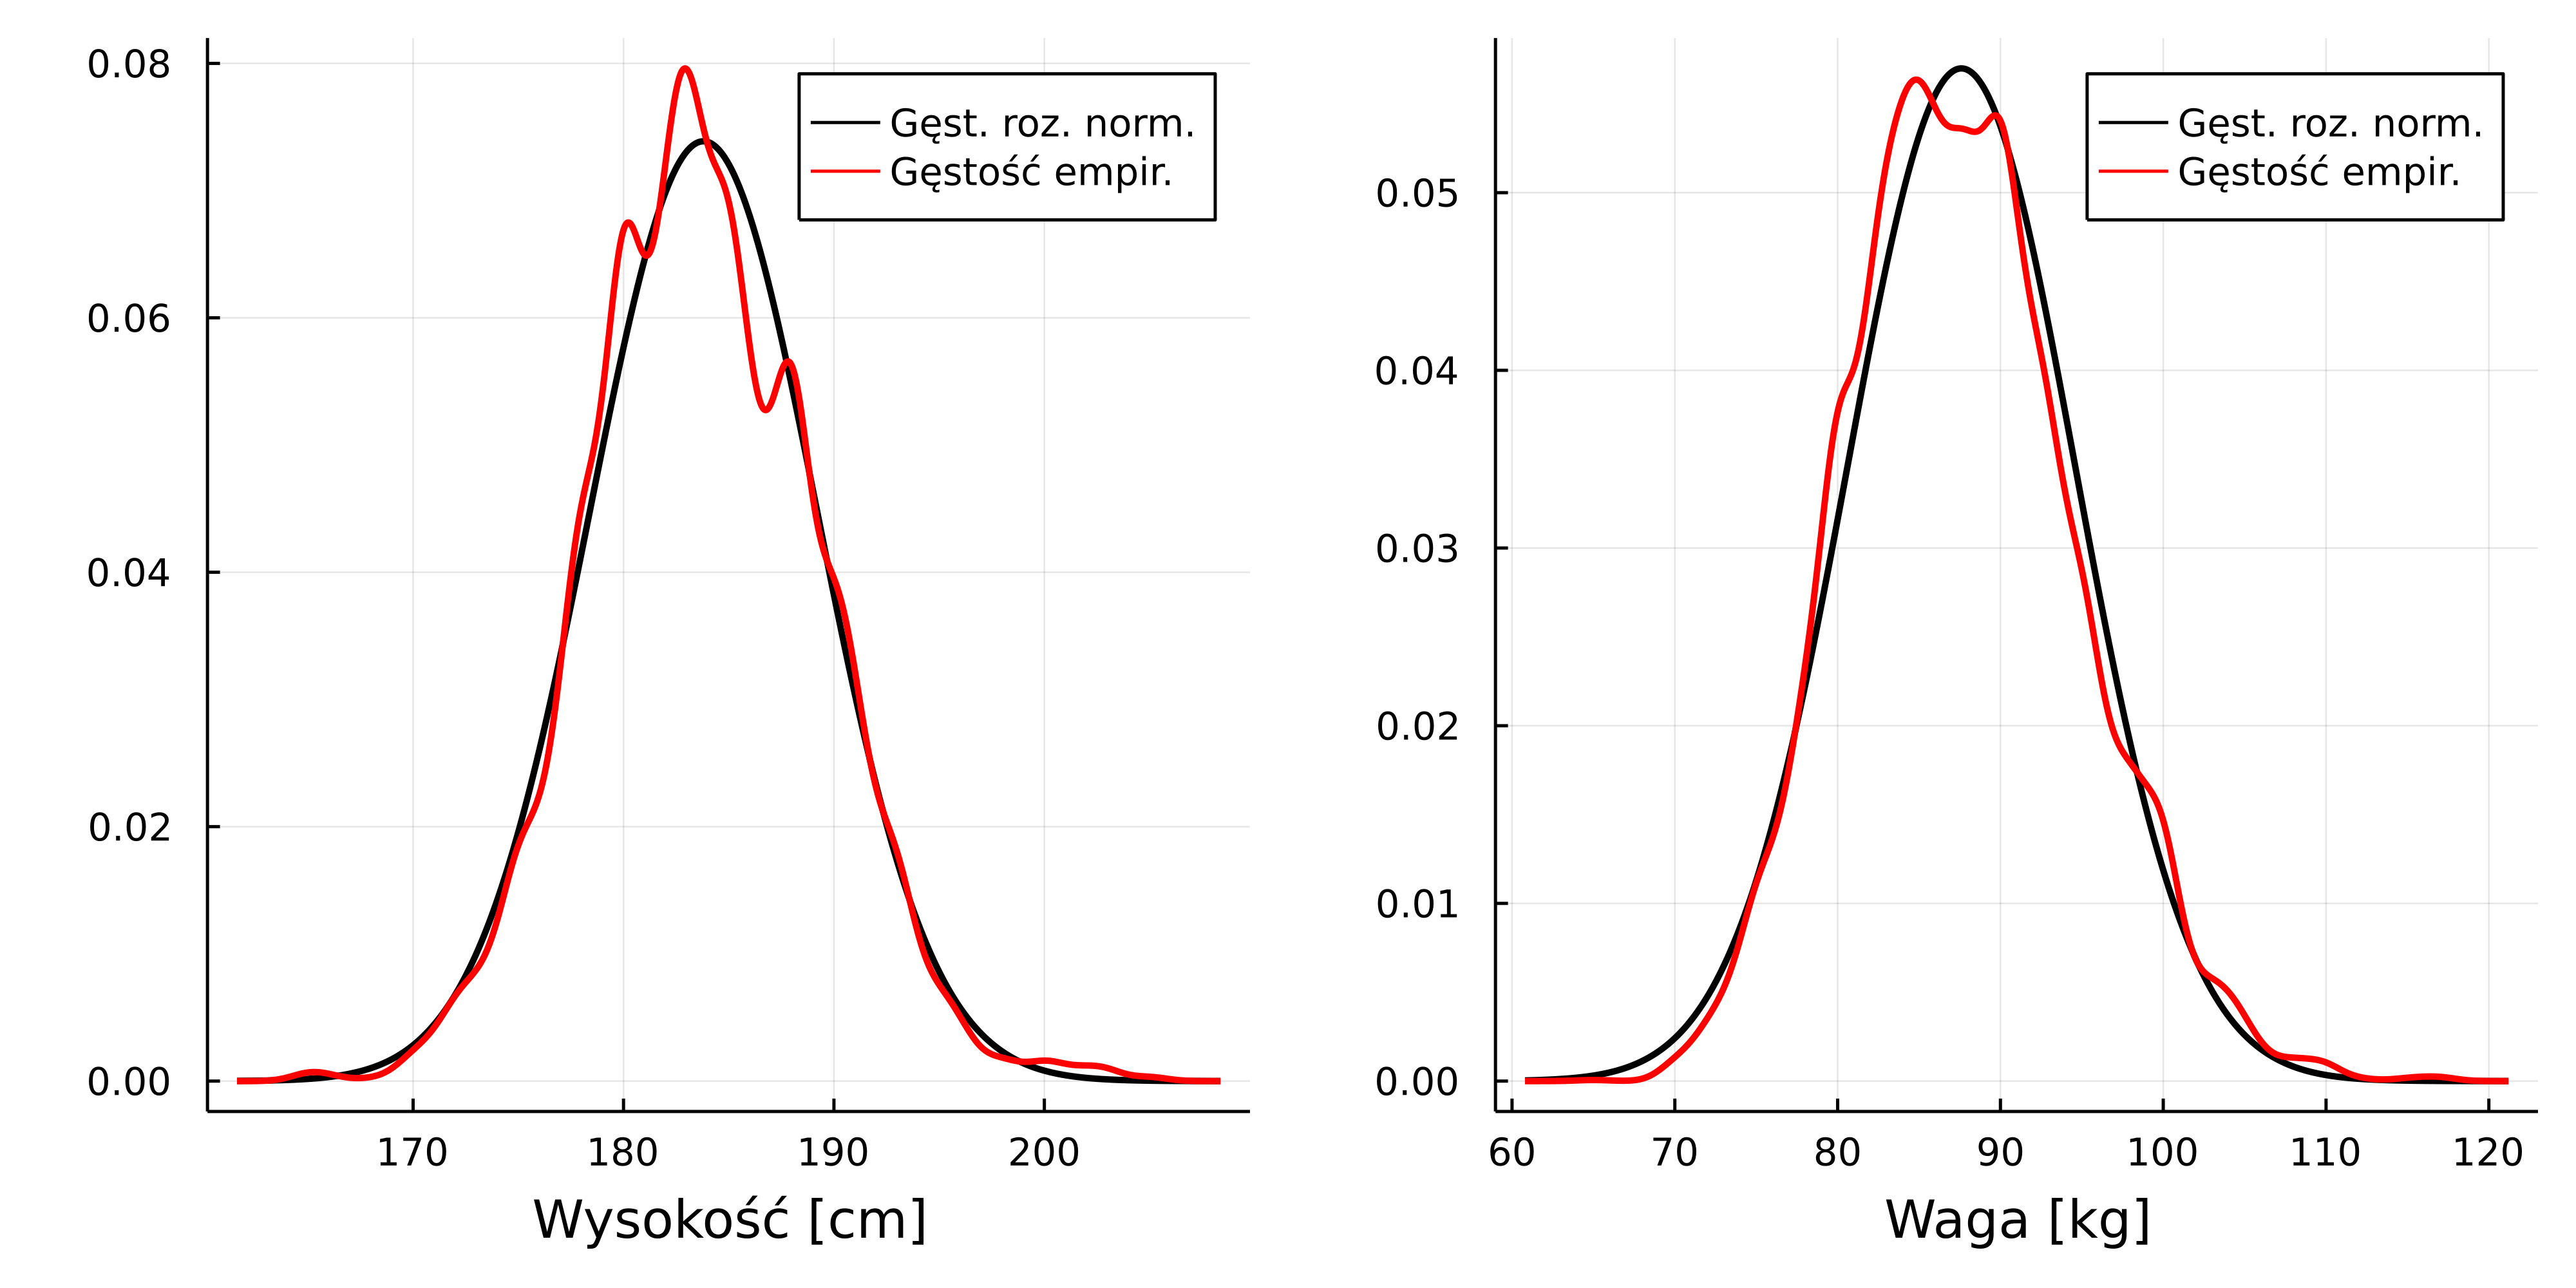
\includegraphics[scale=0.1]{images/normal.png}
		\caption{Porównanie gęstości empirycznej otrzymanej z danych z gęstością rozkładu normalnego $\mathcal{N}(\mu, \sigma)$. Po lewej dla wysokości: $\mu=183,8$, $\sigma=5,4$. Po prawej dla wagi: $\mu=87,6$, $\sigma=7$.}
	\end{figure}
	
	\noindent Okazuje się, że krzywe w obu przypadkach wyraźnie się pokrywają. Dodatkowo dla pewności możemy porównać jeszcze wykresy dystrybuanty empirycznej z dystrybuantą teoretyczną rozkładu normalnego.
	
	\begin{figure}[H]
		\centering
		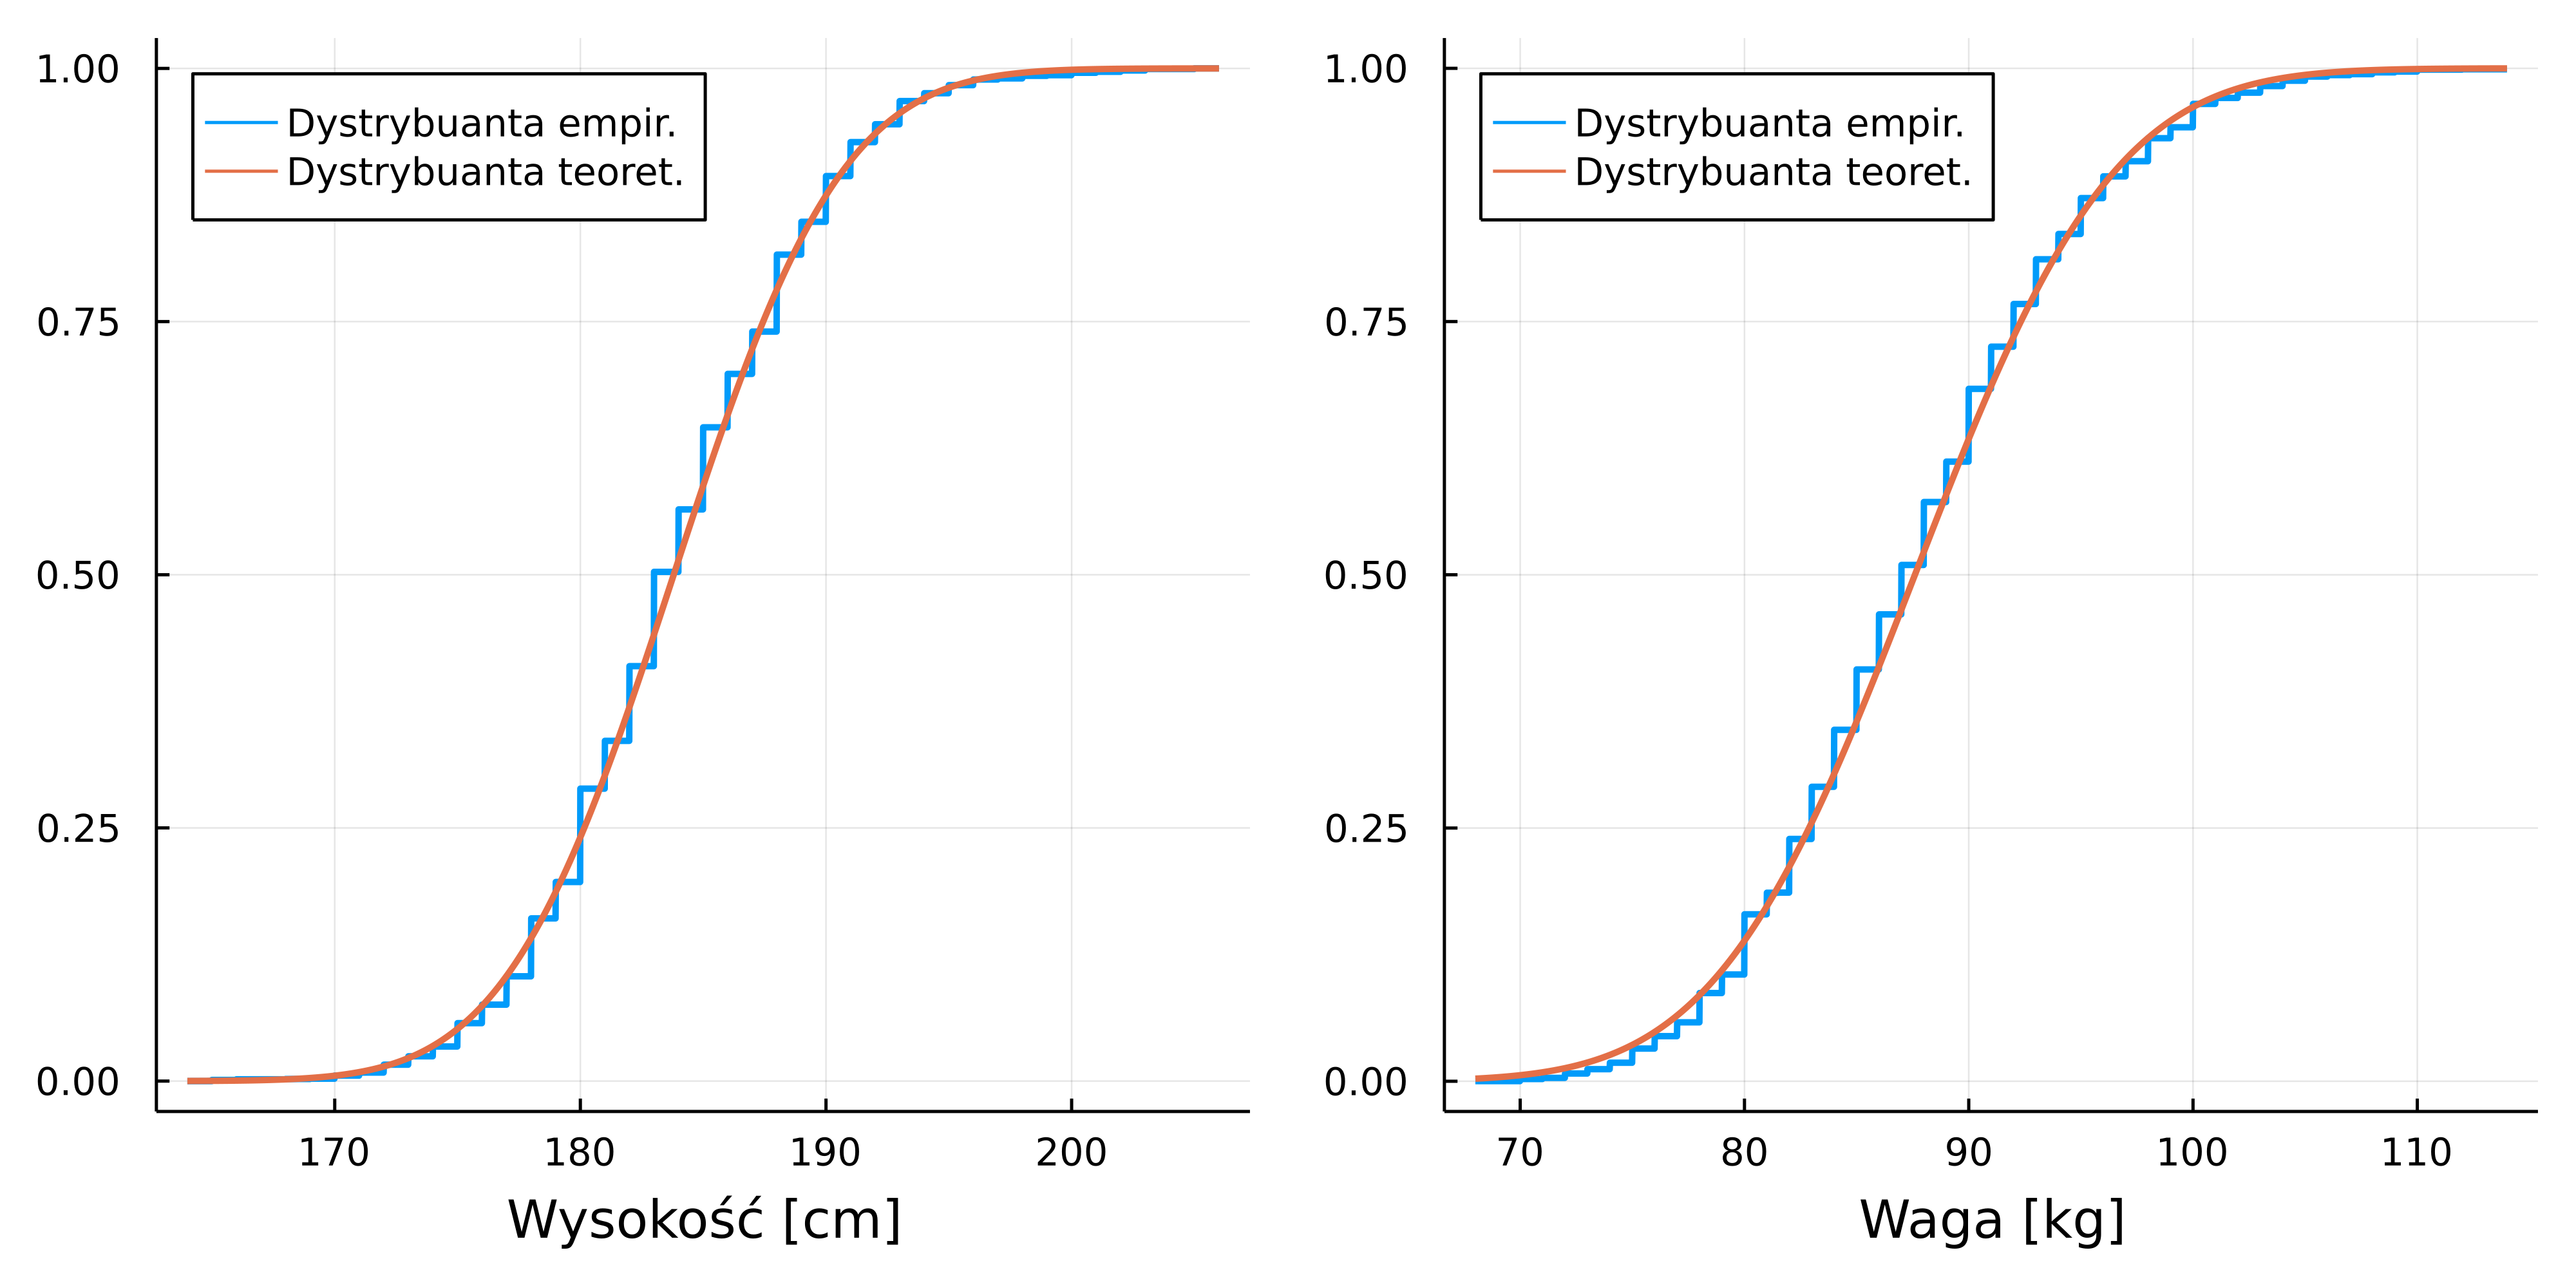
\includegraphics[scale=0.1]{images/ecdf.png}
		\caption{Porównanie dystrybuanty empirycznej otrzymanej z danych z dystrybuantą teoretyczną rozkładu normalnego $\mathcal{N}(\mu, \sigma)$. Po lewej dla wysokości: $\mu=183,8$, $\sigma=5,4$. Po prawej dla wagi: $\mu=87,6$, $\sigma=7$.}
	\end{figure}

	\noindent Podobieństwo krzywych widocznych powyżej potwierdza, że dane pochodzą najprawdopodobniej z rozkładu normalnego lub rozkładu bardzo do niego zbliżonego.
	
	
	\section{Analiza korelacji pomiędzy wagą, a wysokością}
	
	Jak możemy zauważyć na rys. 1, wartości wydają się być od siebie zależne. Nie jest to zaskoczeniem, ponieważ naturalnym jest, że waga zależy od wysokości człowieka. Policzmy współczynnik korelacji Pearsona, by przekonać się jak mocno te dwa zbiory są ze sobą skorelowane. Niech $x_1, \dots, x_n$ oznaczają wysokości, a $y_1, \dots, y_n$ wagi. Wtedy
	$$ r_{xy} = \frac{\sum\limits_{i=1}^{n} x_i y_i - n\bar{x}\bar{y}}{(n - 1) S_x S_y} \approx 0,92, $$
	gdzie $S_x$ i $S_y$ to odchylenia standardowe.
	
	Otrzymaliśmy bardzo wysoką wartość, co oznacza wyraźną korelację. Możemy przypuszczać, że jest tak dlatego, że dane dotyczą sportowców światowej klasy, którzy muszą posiadać odpowiednie parametry fizyczne, by móc startować w zawodach na tak wysokim poziomie. Stąd mamy niewiele odstających danych. W przypadku zwykłych ludzi rozrzut wartości byłby prawdopodobnie znacznie większy, przez co współczynnik korelacji byłby mniejszy.
 	
 	
	\section{Podsumowanie}
	Zgodnie z celem raportu zbadałem zbiór danych opisujący parametry fizyczne zawodników hokeja. Po przyjrzeniu się histogramom oraz wykresom gęstości empirycznej doszedłem do wniosku, że dane mogą pochodzić z rozkładu normalnego, co sprawdziłem porównując gęstość i dystrybuantę empiryczną z gęstością i dystrybuantą teoretyczną rozkładu normalnego. Jako parametry podstawiłem wyliczone wartości średnie oraz wariancje. Okazało się, że rzeczywiście rozkład naszych danych wpasowuje się w rozkład normalny.
	
	Następnie sprawdziłem w jakim stopniu waga i wysokość ze sobą korelują. Otrzymana wartość współczynnika Pearsona wskazuje na znaczną korelację liniową między zbiorami. Stąd wniosek jest taki, że większa wysokość daje lepsze predyspozycje do osiągnięcia większej wagi, co jest w tym sporcie zapewne pożądane, by zawodnik mógł przewracać zawodników drużyny przeciwnej, a nie być przewracanym przez nich.
	
	
	\newpage
	\begin{thebibliography}{1}
		\bibitem{dane}
		\url{https://figshare.com/articles/dataset/Height_of_ice_hockey_players/3394735/2}
	\end{thebibliography}


\end{document}